\documentclass{article}
\usepackage[utf8]{inputenc}
\usepackage[ngerman]{babel}
\usepackage{enumitem}
\usepackage{graphicx}
\usepackage{amsmath}
\usepackage[version=3]{mhchem} 		%% \ce{CO2} -- automatische subscript der zahlen
\usepackage{booktabs}
\usepackage{subfig}
\usepackage{textcomp}
\usepackage{multirow}
\usepackage{fixltx2e}
\usepackage{natbib}
\usepackage{color}

\begin{document}
\title{Kleines Script zur Mikrobiologieklausur}
\author{Christian Müller}

\pagestyle{empty}
\maketitle
\tableofcontents

\pagestyle{headings}
\newpage
\section{Stoffwechsel}
\label{sec:stoffwechsel}
\subsection{Phototrophie}
\begin{description}
	\item[ATP-Produktion]	\hfill \\
	\item[Reduktion von Kohlenstoffdioxid]	\hfill	\\
		mit \ce{NADH} und \ce{NADPH},
		welche durch die vorherige Reduktion von \ce{NAD+} bzw. \ce{NADP*} erzeugt wurden.
\end{description}
	Bei beiden Photosynthesevarianten finden
	verschiedener akzessorischer Proteine und Photosystheme verwendung.
	Dies ermöglich die Anpassung an verschiedene Lebensräume,
	und die Anpassung an die vorhanden Lichtspektren.

\subsubsection{Oxygenen Photosynthese}
	\begin{itemize}
		\item Kein zyklischer Elektronen Transport
		\item Z-Schema mit zwei Photosysteme, (II:P680;I:P700)
	\end{itemize}

\subsubsection{Anoxygene Photosynthese}
	\begin{itemize}
		\item zyklischer Elektronen Transport
		\item Ein Photosystem (P870)
		\item umgekehrter, energieverbrauchender Elektronentransport,
			wenn \ce{NAD(P)H} nötig
	\end{itemize}

\subsubsection{\ce{CO2}-Fixierung}
\begin{description}
	\item[Calvin-Zyklus] ist am weitesten verbreitet.
		Mit den Schlüsselenzymen RUBISCO und Phosphoribulose-Kinase
		erfolgt die Bindung von \ce{CO2} in Glucose
		unter Verbrauch von \ce{ATP} und \ce{NADPH}.
		Siehe Abbildung \ref{fig:calvin_detail}.

	\item[Hydroxypropionat-Weg] der Grünen-Schwefelbakterien.
		Letzlich wird in zwei Zyklen zunächst zwei Moleküle \ce{CO2}
		in Form von Bicarbonat (\ce{HCO3-}) fetgelegt.
		Das Bicarbonat wird dann unter ATP und NADPH Verbrauch zu Glyoxalat aufgebaut.

		Anschließend werden zwei Glyoxalat Moleküle zu Pyruvat umgebaut.

	\item[umgekehrter Citrat-Zyklus] ist die Umkehrung des oxidativen Citratzyklus,
		deshalb auch reduktiver Citrat-Zyklus.
		Die Reaktionen innerhalb des oxidativen Zyklus werden dabei umgekehrt
		unter Umgehung bzw. der Verwenugn spezialisierter Moleküle für die 
		drei Unumkerhbahren Schritte des oxidativen Citrat-Zyklus.

\end{description}

\subsection{Glykolyse (EMP)}
\label{sec:glykolyse}
\begin{itemize}
	\item Ausgeglichene Oxidations-Reduktions-Reaktion
	\item Endprodukt Pyruvat
	\item Ausgangspunk für Fermentation und aerobe Atmung
	\item Weiter Produkte: Reduktionsäquivalent \ce{NADH+}
	\item Verbraucht: 2 ATP
	
\end{itemize}

\begin{enumerate}
	\item Stufe: Vorbereitende Reaktion
	\item Stufe: Synthese von ATP und Pyruvat
	\item Sutfe: Bildung von Fermentationsprodukten, aerobe Atmung
\end{enumerate}

\begin{figure}[htb!]
	\leavevmode
	\begin{center}
		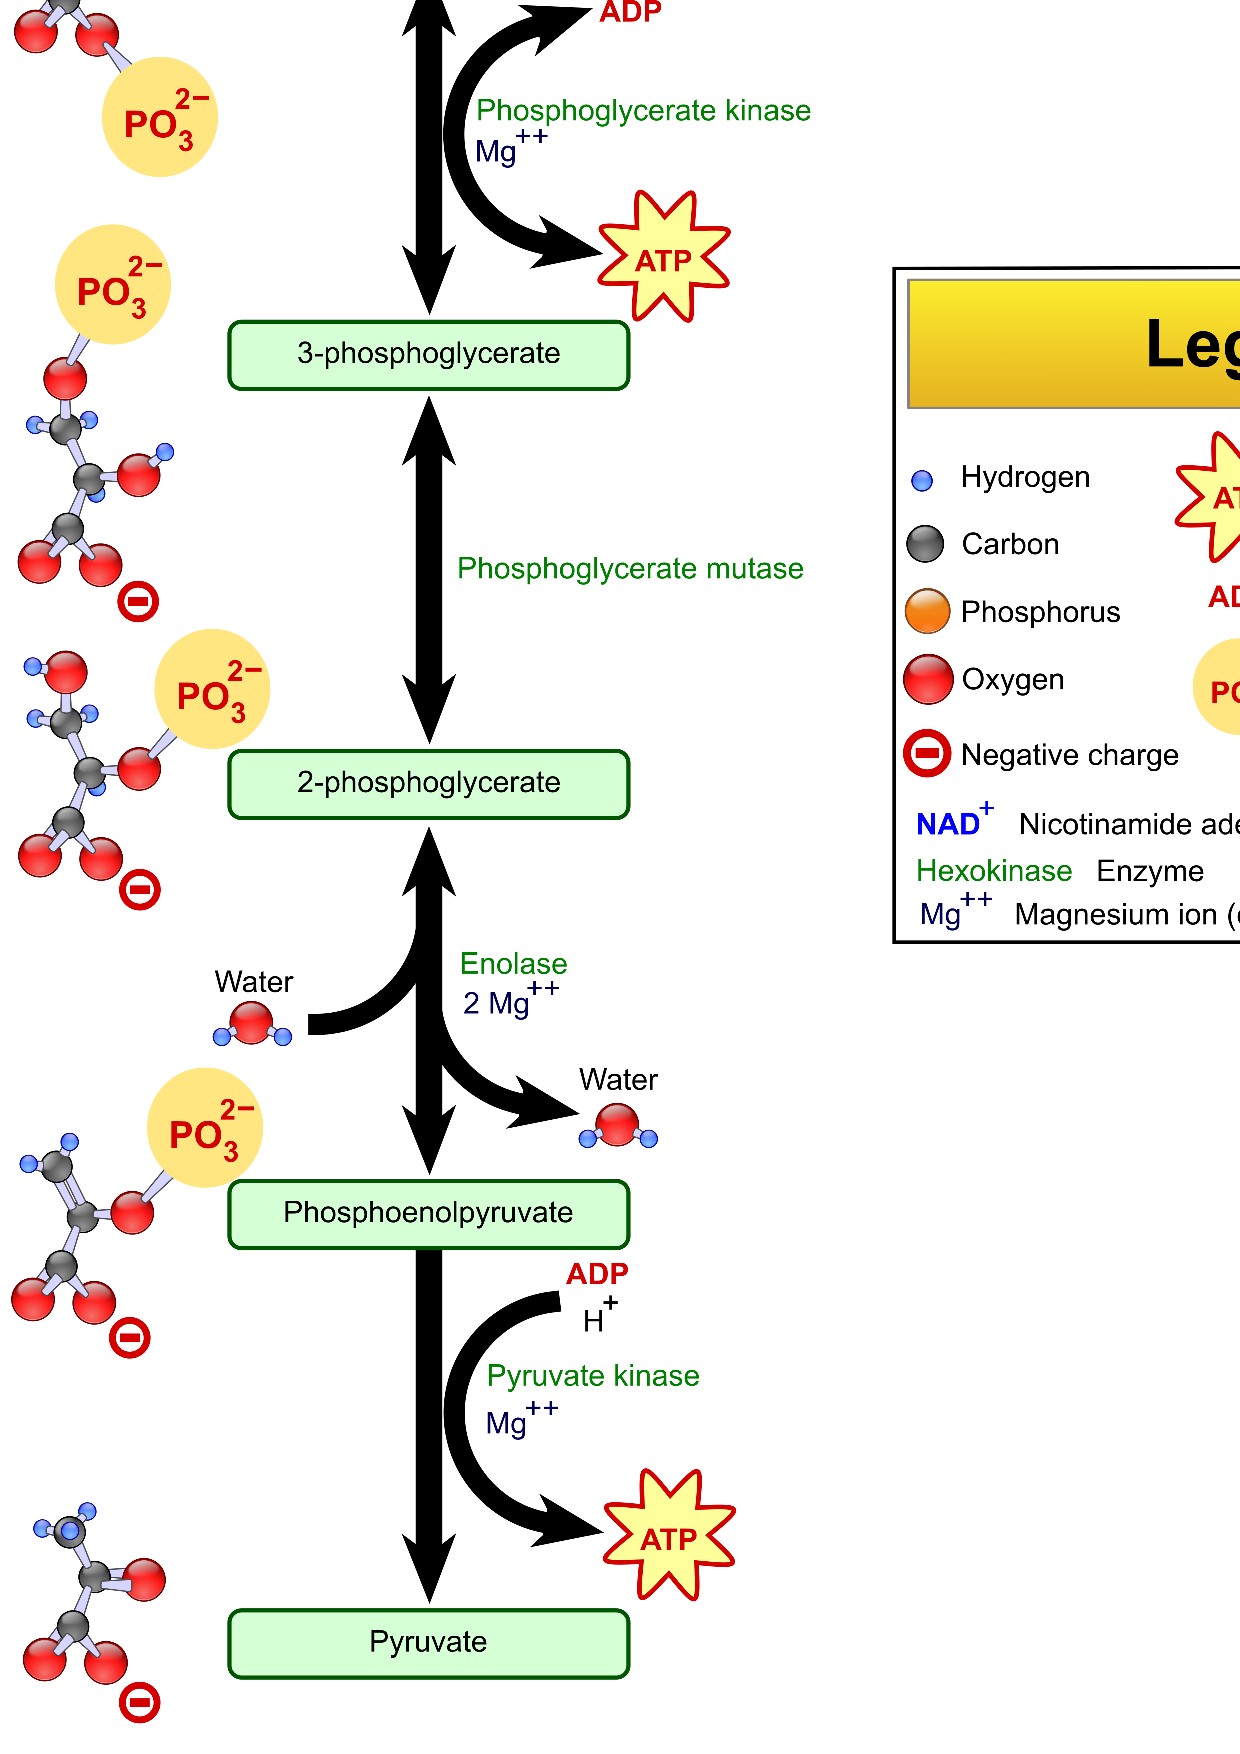
\includegraphics[scale=0.30]{./pictures/glykolysis_2k.pdf}
	\end{center}
	\caption{\slshape{Übersich über die Glykolyse.}}
	\label{fig:glykolyse}
\end{figure}

\subsection{Aerober Stoffwechsel}

\subsubsection*{Aerobe Atmung}
Die Anaerobe Atmung ist ein Stoffwechselvorgang,
zur Energieerzeung.
Durch oxidative biochemische Reaktionen wird dabei ATP erzeugt.
Sie fasst die folgenden Schritte zusammen:

\begin{description}
	\item[Gylkolyse]	\hfill	\\
		Siehe Abschnitt \ref{sec:stoffwechsel}.\ref{secglykolyse} 
		und Abbildung \ref{fig:glykolyse} auf Seite \pageref{fig:glykolyse}
	\item[oxdiative Decarboxylierung]	\hfill	\\
	\item[Citratzyklus]	\hfill	\\
		Siehe Abschnitt \ref{sec:citratzyklus}.
	\item[Endoxidation in der Atmungskette]	\hfill	\\
\end{description}

Die Gesamtbilanz lautet:
\begin{equation}
	\ce{C6H12O6} + 6\ \ce{O2} \rightarrow 6\ \ce{CO2} + 6\ \ce{H2O}
	\label{eq:aerobeAtmung}
\end{equation}

\subsection{Fermentation}

\subsection{Citratzyklus}
\label{sec:citratzyklus}

Der Citratzyklus ist ein zentraler Bestandteil bei der Veratmung organische Verbindungen.

\subsubsection*{Ablauf}
Der C\textsubscript{3}-Körper von Pyruvat wird decarboxyliert,
was zu einem Moleküle \ce{NADH} 
und einem mit dem Coenzym A gekoppelte Acetylmolekül führt.

\begin{figure}[ht!]
	\leavevmode
	\begin{center}
		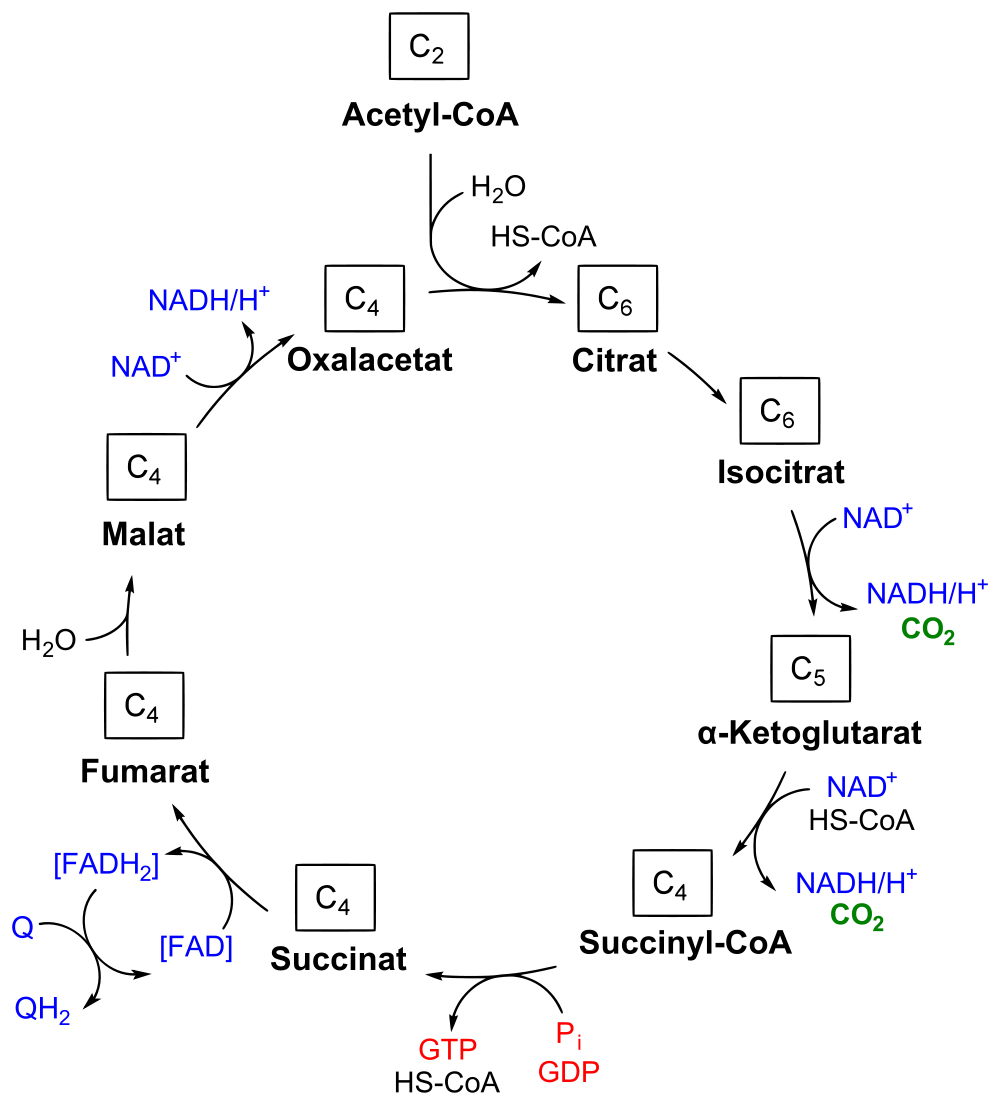
\includegraphics[scale=0.30]{./pictures/citratzyklus_1k}
	\end{center}
	\caption{\slshape{Der Citrat-Zyklus.}}
	\label{fig:calvinDetail}
\end{figure}

Der Citratzyklus wird auch als Tricarbonsäure-Zyklus oder kurz TCA-Zyklus bezeichnet.

\newpage
\section{Biotechnologie}

\begin{description}
	\item[Pasteur-Effekt] \hfill \\
		Mikroorganismen Verstoffwechseln D-Glucose wesentlich stärker in der Gykolyse,
		wenn keine Sauerstoff zur Verfügung steht.
		Der Effekt tritt auch bei der alkoholischen Gärung auf,
		welche aus diesem Grund auch in einer Sauerstofffreien Umgebung durchgeführt wird.

		Bei \emph{S. cerevivsiae} ist der Pasteur-Effekt sehr schwach ausgeprägt,
		was die Hefe für biotechnologische Verfahren interessant macht.

	\item[Alkohol-Produktion] \hfill \\
		Bei der industriellen Herstellung von Ethanol kommt eine ``normale'' gemischte Säuregärung zum Einsatz,
		welche jedoch in Richtung Ethanolproduktion verschoben wird.
		Durch die Eiführung eines ``pet-Operons'' wird die Produktion von Succinat unterbunden.
		Verwendet werden: \emph{S. cerevisiae} und \emph{Zymomonas mobilis}.

	\item[1,3-Propandiol Produktion] \hfill \\
		\begin{itemize}
			\item[Enterobakterien] 
				\emph{Klebsiella pneumononiae},
				\emph{Klebsiella oxytoca},
				\emph{Citrobacter freundii},
				\emph{Citrobacter intermedium}, 
				nicht jedoch \emph{E. coli}
			\item[Clostriedien] 
				\emph{Clostridium pasteurianum},
				\emph{Clostridium butyricum},
				\emph{Clostridium perfingens}
			\item[Andere]
				\emph{Acetobacterium woodii},
				\emph{Acetobacterium carbinolicum},
				\emph{Ilyobacter polytropus},
				\emph{Lactobacillus reuteri},
				\emph{Lactobacillus bervis},
				\emph{Lactobacillus buchneri}
		\end{itemize}

	\item[Prozessoptimierung] \hfill \\
		\begin{itemize}
			\item Screening un Selektion von Stämmen
			\item Gentechnische Veränderung
			\item Optimierung der Bedingungen (Substratzugabe, Produktendtzug, \ldots)
		\end{itemize}

	\item[unvollständige Oxidation] \hfill \\
		Meist mit der Wachstumsphase assoziierte Form der \ce{O2}-Oxidation,
		bei der nicht \ce{CO2} das Ziel ist, sondern ein Zwischenprodukt.

		Durch die unvollständige Oxidation werden biotenologisch hergestellt:
		
		\begin{itemize}
			\item Acetat
			\item Gluconat
			\item Fumarat
			\item Citrat und andere organische Säuren
			\item Aminosäuren
			\item Alkohole
		\end{itemize}

	\item[Biokonversion] \hfill \\
		C-Metabolismus während der stationären Phase. %TODO mehr!

	\item[Sekundär Stoffwechsel] \hfill \\
		Stoffwechsel-Weg zur Erzeugung bestimmter Stoffe die seltener benötigt werden
		(z.B. Antibiotika).

	\item[Tropophase] \hfill \\
		Die Wachstumsphase einer Zelle in der hauptsächlich der Primärmetabolit erzeugt wird.

	\item[Idiophase] \hfill \\
		Die Produktionssphase einer Zelle in der hauptsächlich der Sekundärmetabolit erzeugt wird.

	\item[Angrifforte für Antibiotika] \hfill \\

		\begin{table}[ht!]
		\begin{center}
			\begin{tabular}{p{4cm} p{3cm}} 
		\toprule
			Wirkort	&	Antibiotika \\
			\midrule
			DNS-Replikation		&	Nitroimidazole \\
										&	Fluorcinolone 	\\
			Zellwandbiosynthese	&	\begin{math}\beta\end{math}-Lactame \\
			\multirow{3}{*}{}		&	Glycopeptide 	\\
										&	Bacitaricin 	\\
										&	Cycloserin 		\\
			Folsäurestoffwechsel	&	Trimethoprim	\\
										&	Sulfonamide 	\\
			Proteinbiosynthese	&	Tetracycline \\
			\multirow{5}{*}{}		&	Makrolide 	\\
										&	Aminoglycoside 	\\
										&	Lincosamide 	\\
										&	Oxazolidinone 	\\
										&	Streptogramine 	\\
										&	Chloramphenicol 	\\
			RNS-Polymerase			&	Rifamycine \\
		\bottomrule
		\end{tabular}
		\caption{Angriffsvektoren und die passenden Antiobiotika.}
		\label{tab:wirkorteantibiose}
		\end{center}
		\end{table}

\end{description}

\newpage
\section{Wachstum}

\begin{description}
	\item[Anabolismus] \hfill \\
		Aufbauender, Energie verbrauchender Teil des Metabolismus.
	\item[Katabolismus] \hfill \\
		Abbauende, Energiefreisetzende Reaktion als Teil des Metabolismus.
\end{description}

\subsection{Elemente}

In den Tabellen \ref{tab:makroelemente} und \ref{tab:mikroelemente} befinden sich die
wichtigsten Makro- und Mikroelemente für das mikrobielle Wachstum.

Weiter Wichtige Sustanzen sind Vitamine,
welche von den Mikroorganismen aber auch selbst synthetisiert werden können.

\subsubsection*{Makroelemente}

\ce{CO2} ist bei Autotrophen der Kohlenstoff-Lieferant.

Stickstoff wird meist aus anorganoischen Quellen,
wie Ammoniak, Nitrat oder molekularem Stickstoff (\ce{N2}) gewonnen.

Phosphor ist entshceiden für die Synthese von Nucleinsäuren und Phospholipiden.

Schwefel wird als Strukturgeber für die Aminosäuren Cystein und Methionin, 
sowie Coenyzm A und Kiponsäuren.
Als Quelle dient Sulfat oder Sulfid.

Eisen spielt eine wichtige Rolle in der Atmung.
Es wird für die Cytochrome und Eisenschwefelproteinen beötigt,
wechle beim Elektronentransport mitwirken.

\begin{table}[h!]
	\begin{center}
		\begin{tabular}{l l} 
			\toprule
			Element	&	Bereitstellung	in der Natur \\
			\midrule
			C			&	\ce{CO2}, organische Stoffe \\
			H			&	\ce{H2O}, organische Stoffe \\
			O			&	\ce{H2O}, \ce{O2}, organische Stoffe \\
			N			&	\ce{NH3}, \ce{NO3-}, \ce{N2}, organische Stoffe \\
			P			&	Phosphat \\
			S			&	\ce{H2S}, organische Stoffe, Sulfide \\
			\midrule
			K			&	Kaliumsalze \\
			Mg			&	Magnesiumsalze \\
			Na			&	\ce{NaCl}, Natriumsalze \\
			Ca			&	Salze \\
			\midrule
			Fe			&	\ce{FeS}, Eisensalze \\
			\bottomrule
		\end{tabular}
		\caption{Makroelementen und ihre Quellen für Mikroorganismen}
		\label{tab:makroelemente}
	\end{center}
\end{table}

\subsubsection*{Mikroelemente}

Diese Substanzen weden nur in sehr geringen mengen benötigt,
ihr Vorhandensein ist jedoch entscheiden für das mikrobielle Wachstum.

\begin{table}[h!]
	\begin{center}
		\begin{tabular}{l l} 
			\toprule
			Element	&	Funktion in der Zelle \\
			\midrule
			Co			&	\ce{B12}, Transcaboxylase \\
			Cu			&	Atmung, CytC-Oxidase, Photosynthese\\
			Mn			&	Photosystem II, Superoxiddismutase \\
			Mo			&	Nitrogenase, Nitratreduktase, Formiat-DHG \\
			Ni			&	Hydorgenase, Co-F430 (Methanogene), \ce{CO}-Dehydrogenase \\
			Se			&	Formiat-DHG, Hydrogenase\\
			W			&	Formiat-DHG \\
			V			&	Vanadium-Nitrogenase \\
			Zn			&	Alkohol-DHG, RNA-/DNA-Polymerase \\
			Fe			&	Cytochrome, Katalasen, FeS-Proteine, alle Nitrogenasen \\
			\bottomrule
		\end{tabular}
		\caption{Mikroelementen und ihre Quellen für Mikroorganismen}
		\label{tab:mikroelemente}
	\end{center}
\end{table}

\subsection{Zellteilung}

Bei der Zweiteilung repliziert sich ein Mikroorganismus,
so dass nach dem Prozess zwei gleichwertige Organismen endstanden sind.

\begin{enumerate}
	\item DNA-Replikation
	\item Elongation des Zellkörpers
	\item Septumbildung
	\item Fertigstellung des Septums und Bildung getrennter Zellwände
	\item Trennung der Zellen
\end{enumerate}

Mit der Bildung des FtsZ-Moleküls wird der Prozess angestossen.
Es induziert die DNA-Replikation und Bildet das sogenannte Divisom,
den Zellteilungsapparat.
Der FtsZ-Ring läuft einmal an der Cytoplasmamembran um die Zelle herum und
markiert die Stelle der Trennung.

Der Ring trennt sich auf die beiden endstehenden Zellen auf und
in den Zwischenraum werden die neuen Zellaussenwände eingezogen,
bis das Cytosol der zellen abgeschlossen voneinander ist.

Durch bestimmte Proteine wird am Fts-Ring auch die neuen Zellwandstrukturen gebildet.
Dabei werden die Nahtstellen ``aufgeweicht'' und
verlängert um die Stabilität auch an diesen Stellen zu gewährleisten.

Dieser Prozess des ``Aufweichens'' wird durch Penicillin unterbunden,
was zu einem immer weiteren aufweichen und
damit zur Lyse der zelle führt.

\subsection{Wachstum von Populationen}

\begin{description}
	\item[Generation, Generationszeit] \hfill \\
		Zeit von einer Zweiteilung bis zur darauf Folgenden.

	\item[Exponentielles Wachstum] \hfill \\
		In der exponentiellen Phase vermehren sich bis die 
		Kapazitätsgrenzen erreicht ist und alle Nährstoffe des Habitats sind
		oder ein Stoffwechselprodukt im Medium das Wachstum begrenzt.

	\item[Wachstumsphasen] \hfill \\
		\begin{itemize}
			\item Lag	(+)
			\item Exponentiell	($2^x$)
			\item Satationär	(==)
			\item Absterben	(-)
		\end{itemize}

	\item[Messung] \hfill \\
		Beispielsweise durch Trübung.

\end{description}

\subsection{Umwelteinflüsse auf das Wachstum}

\newpage
\section{Cytologie}

\subsection{Basics}

\begin{itemize}
	\item Domänen: Bacteria, Archaea und Eukarya
	\item Verhältnis Oberfläche/Volumen 
	\item Gramfärbung benötigt Kristallviolett (g+) und Safranin (g-),
		zwischendurch Entfärbung von Kristallviolett mit Ethanol.
		Ethanol verschließt Peptidoglycanschicht von Grampositiven,
		deshalb wird die Farbe nicht entzogen.
	\item Haupttypen der Morphologie: 
		Kokken,
		Stäbchen,
		Spirillen,
		Spirochäten,
		Knospende Bakterien,
		Bakterien mit Zennanhängen
		und filamentöse Bakterien
\end{itemize}

\begin{description}
	\item[gram-positiv]
		Eigenschaft einer prokaryotischen Zelle,
		deren Zellwand vorallem aus Peptidoglycan besteht
		und der die äußere Membran von gram-negativen Zellen fehlt.

	\item[gram-negativ] 
		Eigenschaft einer prokrayotischen zelle,
		deren Zellwand geringe Mengen von Petidoglycan enthält.
		Sowie eine äußere Membran,
		die Lipopolysaccahride,
		Lipoproteine,
		und andere komplexe Makromoleküle enthält.

	\item[Peptidoglycan]
		Polysaccharid,
		das aus alternierenden Wiederholungen von Acetyglucosamin und Actylmuraminsäuren besteht,
		die in benachbarten Shichten angeordnet
		und durch kurze Peptide quervernetzt sind.

\end{description}

In Tabelle \ref{tab:domaenenuberblick} ist eine Übersich über die Eigenschaften der drei Organismenreiche.	

\begin{table}[h!]
	\begin{center}
		\begin{tabular}{l l l l} 
			\toprule
			Merkmal		&	Bacteria		&	 Archaea				&	 Eukaraya		\\
			\midrule
			Zellkern 	&	nein			&	 nein					&	 ja		\\
			cccDNA		&	ja				&	 ja					&	 nein (linear)			\\
			Histone		&	nein			&	 ja					&	 ja		\\
			Zellwand		&	Murein		&	 kein Murein		&	 kein Murein		\\
			Membranlipid&	Ester			&	 Ether				&	 Ester		\\
			\midrule
			Ribosomen	&	70S			&	 70S					&	 80S		\\
			Ini-tRNA		&	f-Met			&	 Met					&	 Met		\\
			Introns 		&	nein			&	 nein					&	 ja		\\
			ja				&	Operon		&	 ns					&	 nein		\\
			Cap/poly-A 	&	nein			&	 nein					&	 ja		\\
			Plasmide		&	ja				&	 ja					&	 selten		\\
			RNA-Pol			&	ne (4 UE)	&	 viele (8-12 UE)	&	drei (12-14 UE)	\\
			TK-Faktoren		&	nicht nötig	&	 benötigt			&	benötigt		\\
			Promotoren		&	-10, -35		&	 TATA					&	TATA		\\
			\midrule
			Methanbildung		&	nein			&	 ja					&	nein		\\
			S-Reduktion		&	ja				&	 ja					&	nein		\\
			Nitrifizierung	&	ja				&	 nein					&	nein		\\
			Denitrifizierung		&	ja				&	 ja					&	nein		\\
			N-Fixierung		&	ja				&	 ja					&	nein		\\
			Photosynthese		&	ja				&	 nein					&	nein (Plastiden)	\\
			Lithotrophie	&	ja				&	 ja					&	nein		\\
			Grw. > 80°C		&	ja				&	 ja					&	nein		\\
			\bottomrule
		\end{tabular}
		\caption{Übersicht über die Eigenschaften der drei Organismenreiche.}
		\label{tab:domaenenuberblick}
	\end{center}
\end{table}

\subsection{Aufbau}

\subsubsection{Eukarya}
\begin{figure}[ht!]
	\leavevmode
	\begin{center}
		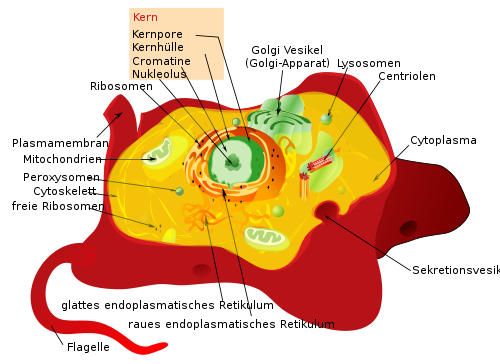
\includegraphics[scale=0.47]{./pictures/animal_cell_500}
	\end{center}
	\caption{\slshape{Tierische Zelle als Beispiel einer eukaryotischen Zelle.}}
	\label{fig:eukarya}
\end{figure}

\subsubsection{Prokarya}
\begin{figure}[ht!]
	\leavevmode
	\begin{center}
		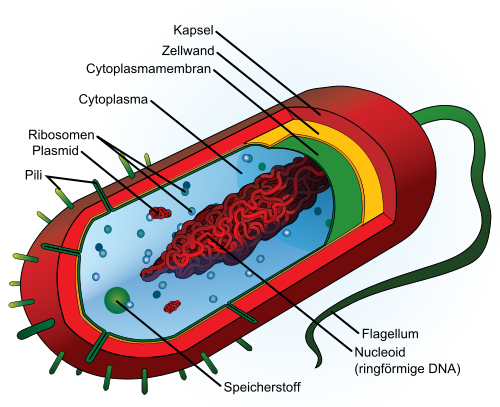
\includegraphics[scale=0.47]{./pictures/avg_prokaryote_cell_500}
	\end{center}
	\caption{\slshape{Typische prokaryotische Zelle.}}
	\label{fig:prokarya}
\end{figure}

\subsubsection{Endosporen}

\begin{itemize}
	\item Überdauerungstadium
	\item steigert Resistenz gegen schädliche äußere Einflüsse
	\item kein/kaum Metabolismus
	\item Reduktion des Wassergehaltes auf 10-25\% im Kern
	\item meist von gram-positive Zellen, auch einige gram-negative
\end{itemize}

\subsubsection{Bewegung mit Geißeln}

\begin{description}
	\item[Aufbau] \hfill \\
		Der typische Aufbau ist in Abbildung \ref{fig:flagellum},
		für ein Gram-negatives Bakterium dargestellt.

		Das Flagellum selbst besteht aus Untereinheiten des Moleküls Flagllin.
		Der Haken ist aus einem einzigen Protein und verbindet den ``Motor'' mit dem Filament.

		Der Motor ist mit Rotor und Stator in die Zellwand eingelassen,
		wobei er alle Schichten durchdringt.
		Der Stator ist Bestandteil der Cytoplasmamembran.
		
		Bestandteile des Rotos sind:
		\begin{description}
			\item[L-Ring] Lipopolysaccharidschicht
			\item[P-Ring] Petidoglycanschicht
			\item[MS-Ring \& C-Ring] Cytoplasmamembran und Cytoplasma
		\end{description}

		Zwischen MS- und C-Ring befinden sich Fli-Proteine,
		welche mit dem Mot-Protein die Bewegung vermitteln.

		\begin{figure}[ht!]
			\leavevmode
			\begin{center}
				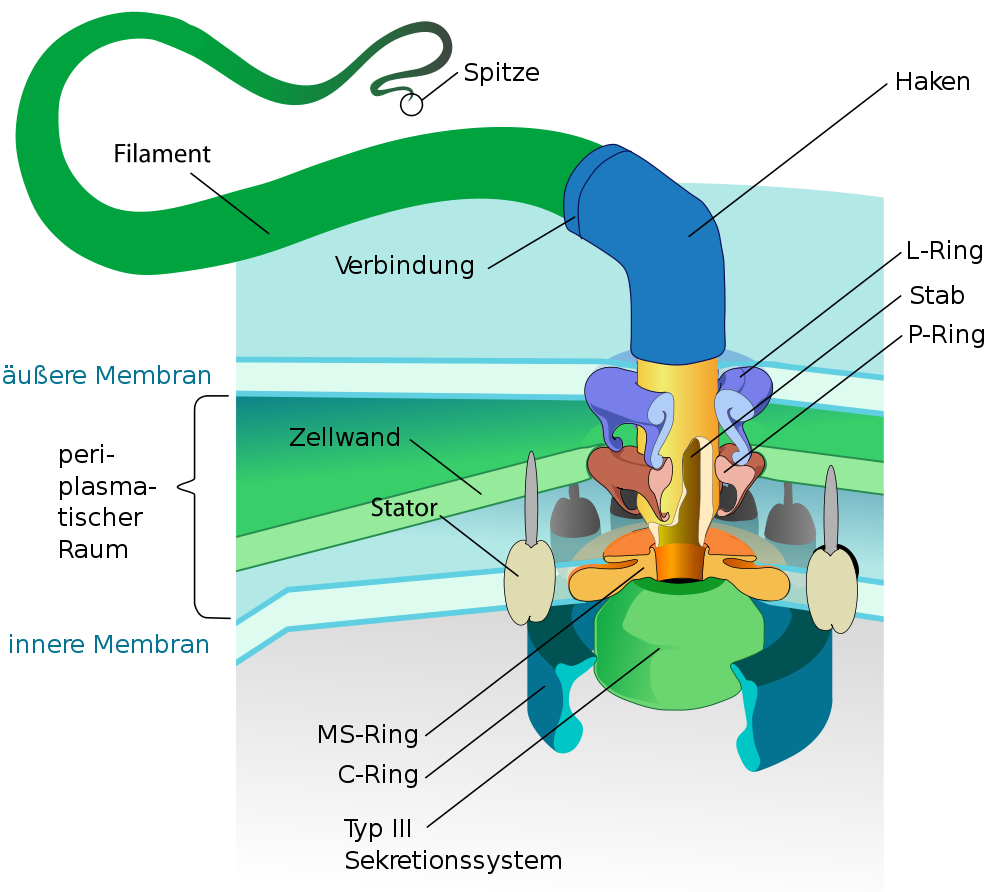
\includegraphics[scale=0.3]{./pictures/flagellum_1k}
			\end{center}
			\caption{\slshape{Motorkomplex eines Gram-negativen Bakteriums.}}
			% http://de.wikipedia.org/w/index.php?title=Datei:Flagellum_base_diagram_de.svg&filetimestamp=20110817105413
			\label{fig:flagellum}
		\end{figure}

	\item[Ablauf der Bewegung] \hfill \\
		Getrieben duch die Protonenmotorische Kraft,
		strömen \ce{H+} durch das Mot-Protein.
		Durch die versetzte Anordnung von positiven und negativen Ladungen auf den Ringen,
		und den Durchstrom der positiven Ladung,
		wird eine Drehbewegung über die Ringe auf den Schaft des Flagllums übetragen.

		Die Geschwindigkeit kann bis zu 60 Körperlängen/Sekunde erreichen,
		ein Gepard erreicht nur 25 Körperlängen/Sekunde.

	\item[Synthese] \hfill \\
		Zunächst wird der MS-Ring synthetisiert und schiebt sich in die Cytoplasmamembran.
		Dann werden die Motorproteinen und die Ringe bis zum Hacken synthetisiert.
		Anschließend bildet sich eine Kappe am Ende Des Hackens.
		Zwischen hacken und der Kappe werden nun Flagelin Proteine eingebaut,
		welche durch einen Kanal vom Cytoplasma in Richtung Kappe fließen.

		Abgebrochene Filamente können so auch repariert werden.

	\item[Steuerung] \hfill \\
		Wiederhole:
		\begin{enumerate}
			\item gebündelte Geißeln zur Fortbewegung in eine Richtung
			\item zertstreute Geißeln zum Taumeln und Neu-Orientieren
			\item gebündelte Geißeln zur Fortbewegung in eine Richtung
		\end{enumerate}

	\item[Orientierung] \hfill \\
		Die Orientierung erfolg oft anhand von Gradieten,
		typischerweise chemische oder Helligkeitsgradienten.
		
		\begin{description}
			\item[Chemotaxis]	Orientierung zu einem Konzentrationsgradienten.
				Laufenden Messung der Konzentration durch Chemorezeptoren,
				bei Abnahme oder Konstantem Wert, taumeln und neu orientieren.
				Sonst Weiter gradeaus.
			\item[Phototaxis] Orientierung an der Helligkeit/Lichspektrum.
				Photopigmente messen Spektrum, sonst wie Chemotaxis.
		\end{description}
		
		Weitere, ähnliche Taxien sind: 
		\begin{description}
			\item[Aerotaxis]	Sauerstoff
			\item[Osmotaxis]	Konzentration hoher Ionenstärke
		\end{description}

		Der Ablauf ist prinzipielle dem der Chemotaxis sehr ähnlich
		Der Ablauf ist prinzipielle dem der Chemotaxis sehr ähnlich..
\end{description}

\subsection{Membran}
\begin{description}
	\item[Einheitsmembranen (unit membrane)] \hfill \\
		\begin{itemize}
			\item Doppelschicht aus amphiphilen Fettsäuren (8 nm)
			\item ungesättigte Fettsäuren führen zu erhöhter Fluidität
			\item Temperaturanpassung, fluider: Cholesterin (Eukarya)
			\item Temperaturanpassung, starrer: Sterole (Eukarya), Hopanoide (Prokarya), nicht in Archaea
			\item Archaea: Ether- statt Esther-Bindung zwischen Glycerin und hydrophoben Seitenketten; 
				Isopren-ketten statt Fettsäuren; Auch: Monolayer durch verknüpfte Lipide
			\item Funktion: Permeabilitätsbarriere, Proteinverankerung, Energiekonservierung
		\end{itemize}

	\item[Äußere Membran (outermembrane)] \hfill \\
		\begin{itemize}
			\item Peptidoglycanschicht
			\item Periplasma
		\end{itemize}

	\item[Transport] \hfill \\
		\begin{itemize}
			\item Einfacher Transport, getrieben durch protonenmotorische Kraft
			\item Gruppentranslokation, chemische Veränderung der transportierten Verbindung,
				getrieben durch Phophoenolpyruvat
			\item ABC-System, mit Permiplasmatischen Bindeproteinen,
				getrieben durch ATP
		\end{itemize}

	\item[Grampositive Zellwand] \hfill \\
		Cytoplasmamembran mit aufgelagerter Peptidoglycanschicht.
		Beide Schichten enthalten Membranproteine.
		Verbindung durch Lipoteichonsäuren,
		die durch die Peptidoglycanschicht bis in die Cytoplasmamembran reichen.
		Teichonsäuren reichen nur in die Peptidoglycanschicht.

		\begin{figure}[ht!]
			\leavevmode
			\begin{center}
				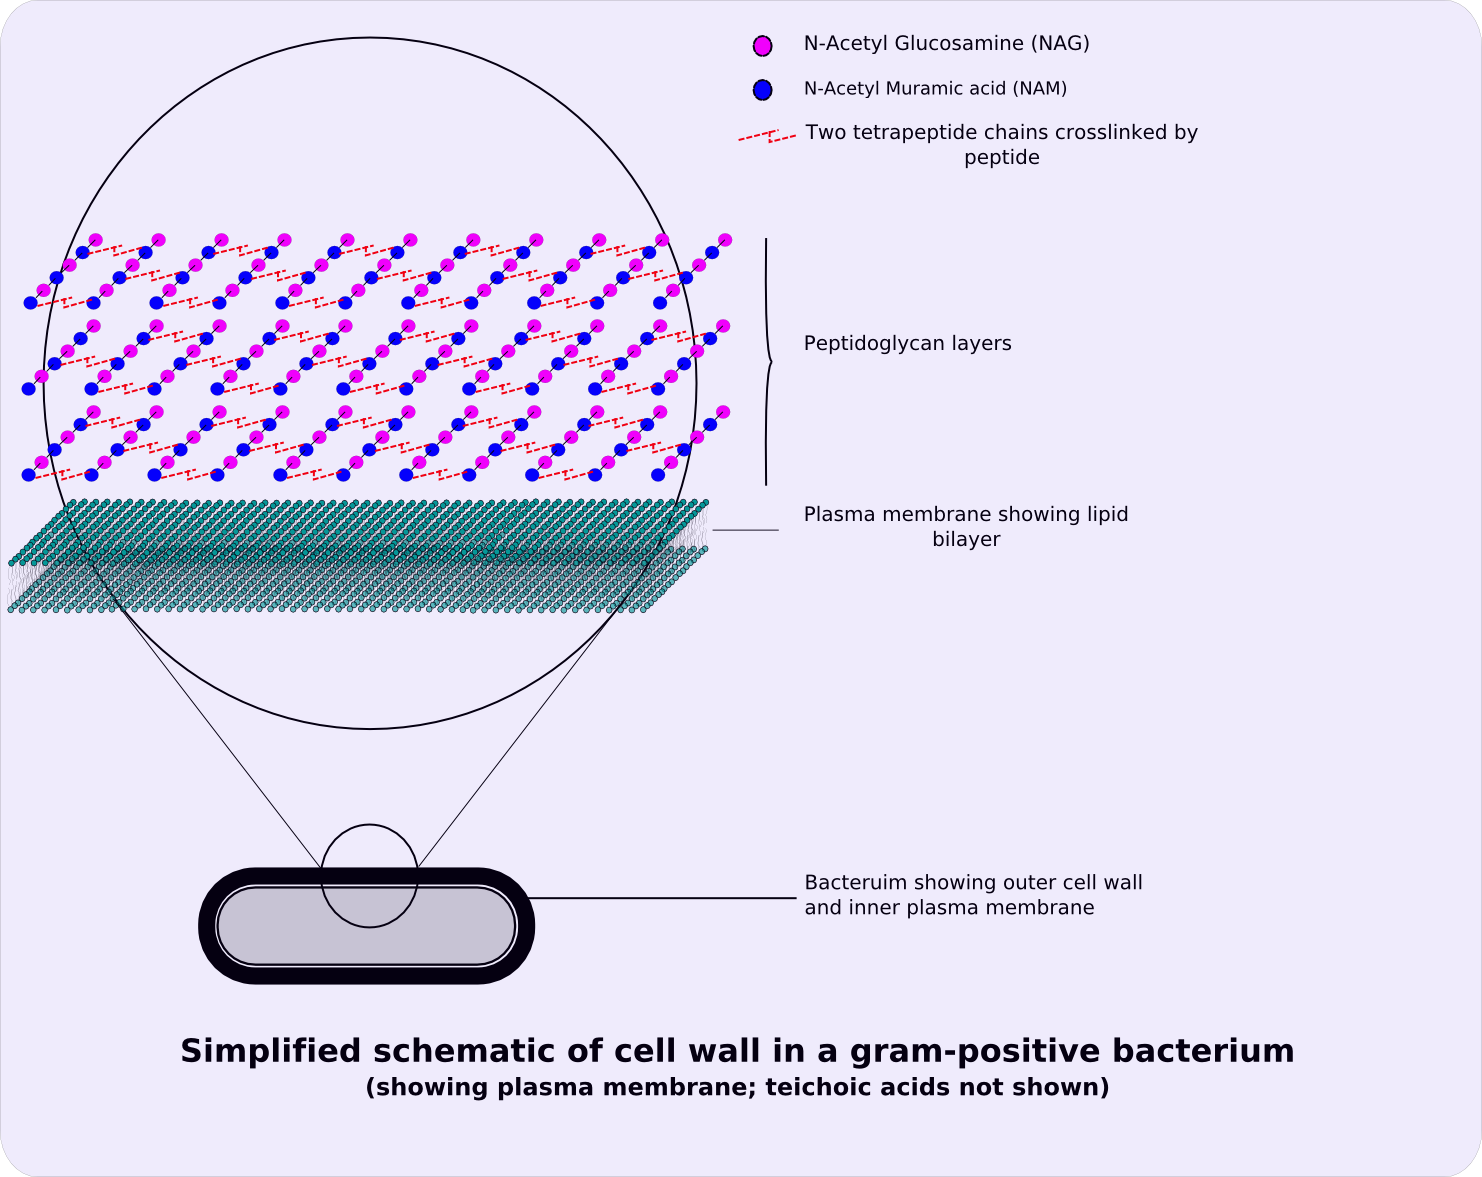
\includegraphics[scale=0.27]{./pictures/gram_positive_zw}
			\end{center}
			\caption{\slshape{Gram-Positive Zellwand der Bacteria.}}
			\label{fig:gramPosBacZW}
		\end{figure}

	\item[Gramnegative Zellwand] \hfill \\
		Zusätzlich zum Peptidoglycan eine Zusätzliche Äußere Membran.
		Sie ist aufgebaut wie die Cytoplasmamembran,
		enthält jedoch zusätzlich Polysaccharide,
		welche einen sogenannten Lipopolysaccharidkomplex bilden,
		daher auch Lipopolysaccharidschicht (LPS).

		Die Lipooplysaccharide sind dabei auf die äußere Membran aufgelagert
		und beinhaltet ebenfalls Transportproteine.
		Der Zwischenraum ober und unterhalb des Peptidoglycanschicht 
		wird als Periplasma bezeichnet.
		Die Verankerung der LPS erfolgt durch Lipoproteine mit der Peptidoglycanschicht.

		\begin{figure}[ht!]
			\leavevmode
			\begin{center}
				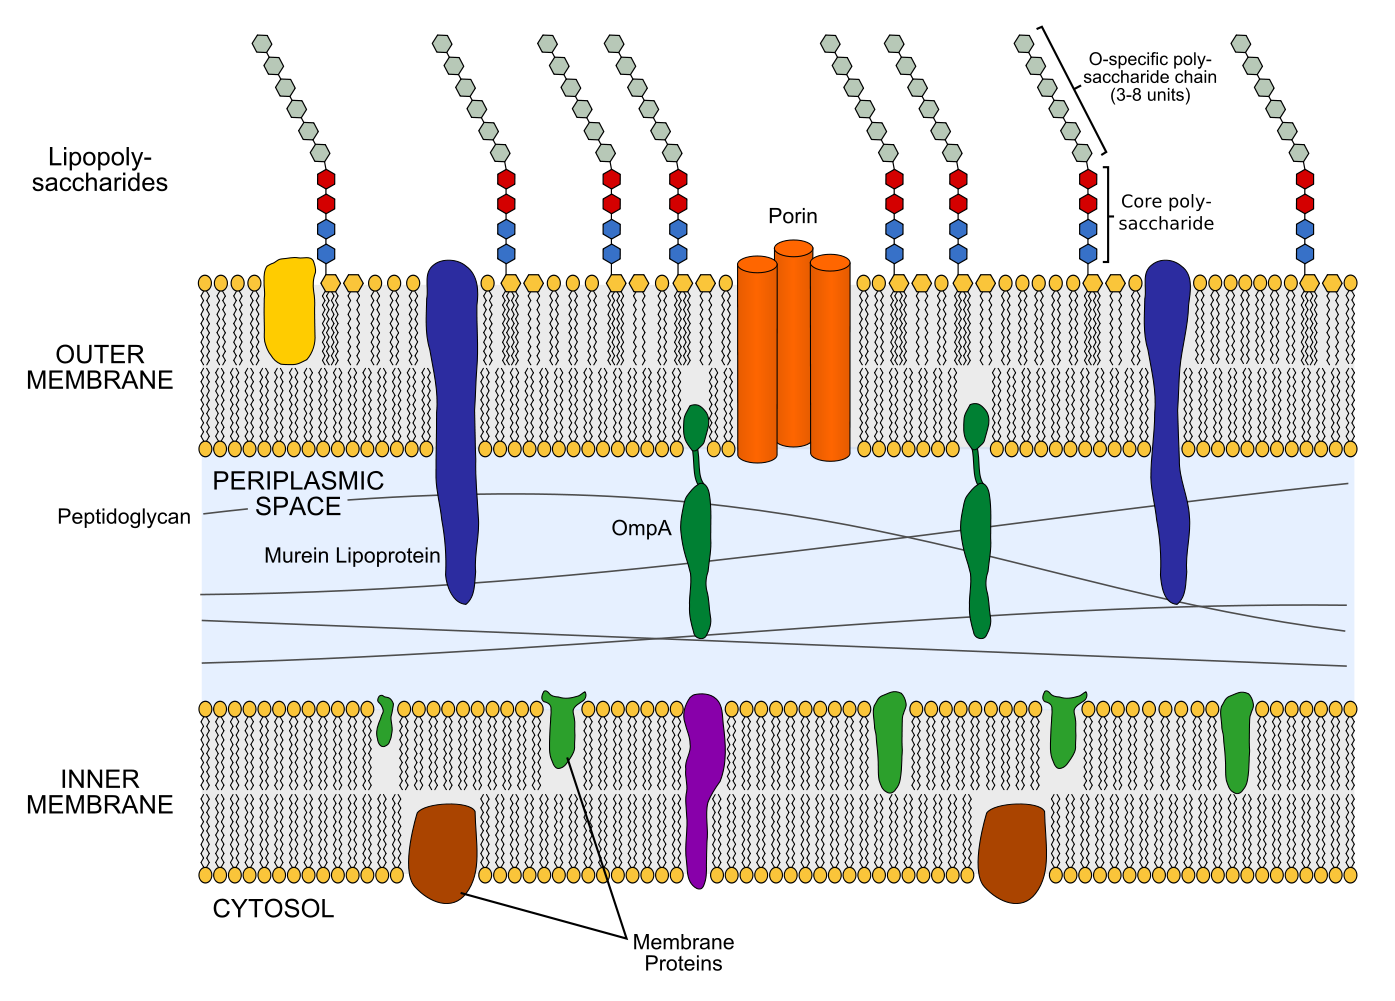
\includegraphics[scale=0.25]{./pictures/gram_negative_zw_noLegend}
			\end{center}
			\caption{\slshape{Gram-Negative Zellwand der Bacteria.}}
			\label{fig:gramNegBacZW}
		\end{figure}
\end{description}

\subsection{Zellwand}

\newpage
\section{Begriffe}

%TODO Verweise auf die Sektionen

\begin{description}
	\item[aerob/anaerob]\hfill \\
		Abhängigkeit des Stoffwechsels von Sauerstoff.

	\item[Autotrophie] \hfill \\
		\ce{CO2} als Quelle für Kohlenstoff.
		(Auch: Primäproduzenten)

	\item[Chemolithotrophie]\hfill \\
		Energiegewinnung aus Oxidation anorganischer Substanzen.
		Nur bei Prokaryoten.
		(Auch: Chemoautotrophie)\\
		Beispielsweise: \textbf{\ce{H2}} + \ce{O2} \textrightarrow  \ce{H2O} + \textbf{ATP}

	\item[Chemoorganotrophie]\hfill \\
		Energirgewinnung aus Oxidation organischer Stoffe.\\
		Beispielsweise: \textbf{Glucose} + \ce{O2} \textrightarrow  \ce{CO2} + \ce{H2O} + \textbf{ATP}

	\item[Fermentation] \hfill \\
		Anaerober Katabolismus, bei dem eine organische Verbindung sowohl
		Elektronendonator als auch Elektronenakzeptor dient und bei dem
		ATP durch Substratkettenphosphrylierung gebildet wird.

	\item[Glykolyse] \hfill \\
		Ein biochemischer Weg,
		bei dem Glucose fermentiert wird und ATP sowie verschiedenen
		Fermentationsprodukte gebildet werden.
		(Auch: ``Embden-Myerof-Weg'')

	\item[Heterotrophie] \hfill \\
		Abhängigkeit von mehrern Kohlenstoffquellen.
		Zumeist Chemolithotrophe.

	\item[Oxidationsstufen] \hfill \\
		\begin{table}[h!]
		\begin{center}
		\begin{tabular}{l l} 
			\toprule
			Element			&	Summenformel		\\
			\midrule
			\multicolumn{2}{l}{Schwefel}			\\
			Sulfid			&	\ce{S}$^{2-}$		\\
			Sulfit			&	\ce{SO3}$^{2-}$	\\
			Sulfat			&	\ce{SO4}$^{2-}$	\\
			Thiosulfat		&	\ce{S2O3}$^{2-}$	\\
			\midrule
			\multicolumn{2}{l}{Stickstoff}		\\
			Nitrit			&	\ce{NO2}$^{-}$		\\
			Nitrat			&	\ce{NO3}$^{-}$		\\
			\bottomrule
		\end{tabular}
		\caption{Übersicht über die Oxidationsstufen von Schwefel.}
		\label{tab:oxidationsstufen}
		\end{center}
		\end{table}

	\item[oxidative Poshorylierung] \hfill \\
		Bildung von ATP auf Kosten der protonenmotorischen Kraft,
		die durch Elektronentransport erzeugt wird.

	\item[Photophosphorylierung] \hfill \\
		Bildung von ATP durch die protonenmotorische Kraft,
		die durch lichtangetrieben Elektronentransport erzeugt wird.

	\item[Phototrophie]\hfill \\
		Energirgewinnung durch Licht.\\
		Bei der Oxgenen Photosynthese endsteht Sauerstoff als Abfallprodukt,
		bei der Anoxygenen nicht.
		Phototrophe Organismen sind meinst auch Autotroph.
		Licht \textrightarrow ATP

	\item[protonenmotorische Kraft] 	\hfill	\
		Ein energetisierter Zustand der Membran,
		der durch die Trennung von Ladung und den Elelemten des Wassers
		($H^+$ und  $OH^-$) über die Membran endsteht.

	\item[Reduktionspotenzial ($E_0'$)] \hfill \\
		Die einer Verbindung innewohnenden Neigung,
		gemessen in Volt,
		unter Standartbedingungen,
		Elektronen abzugeben.

	 \item[Stoffwechsel] \hfill \\

		\begin{figure}[ht!]
		\leavevmode
		\begin{center}
		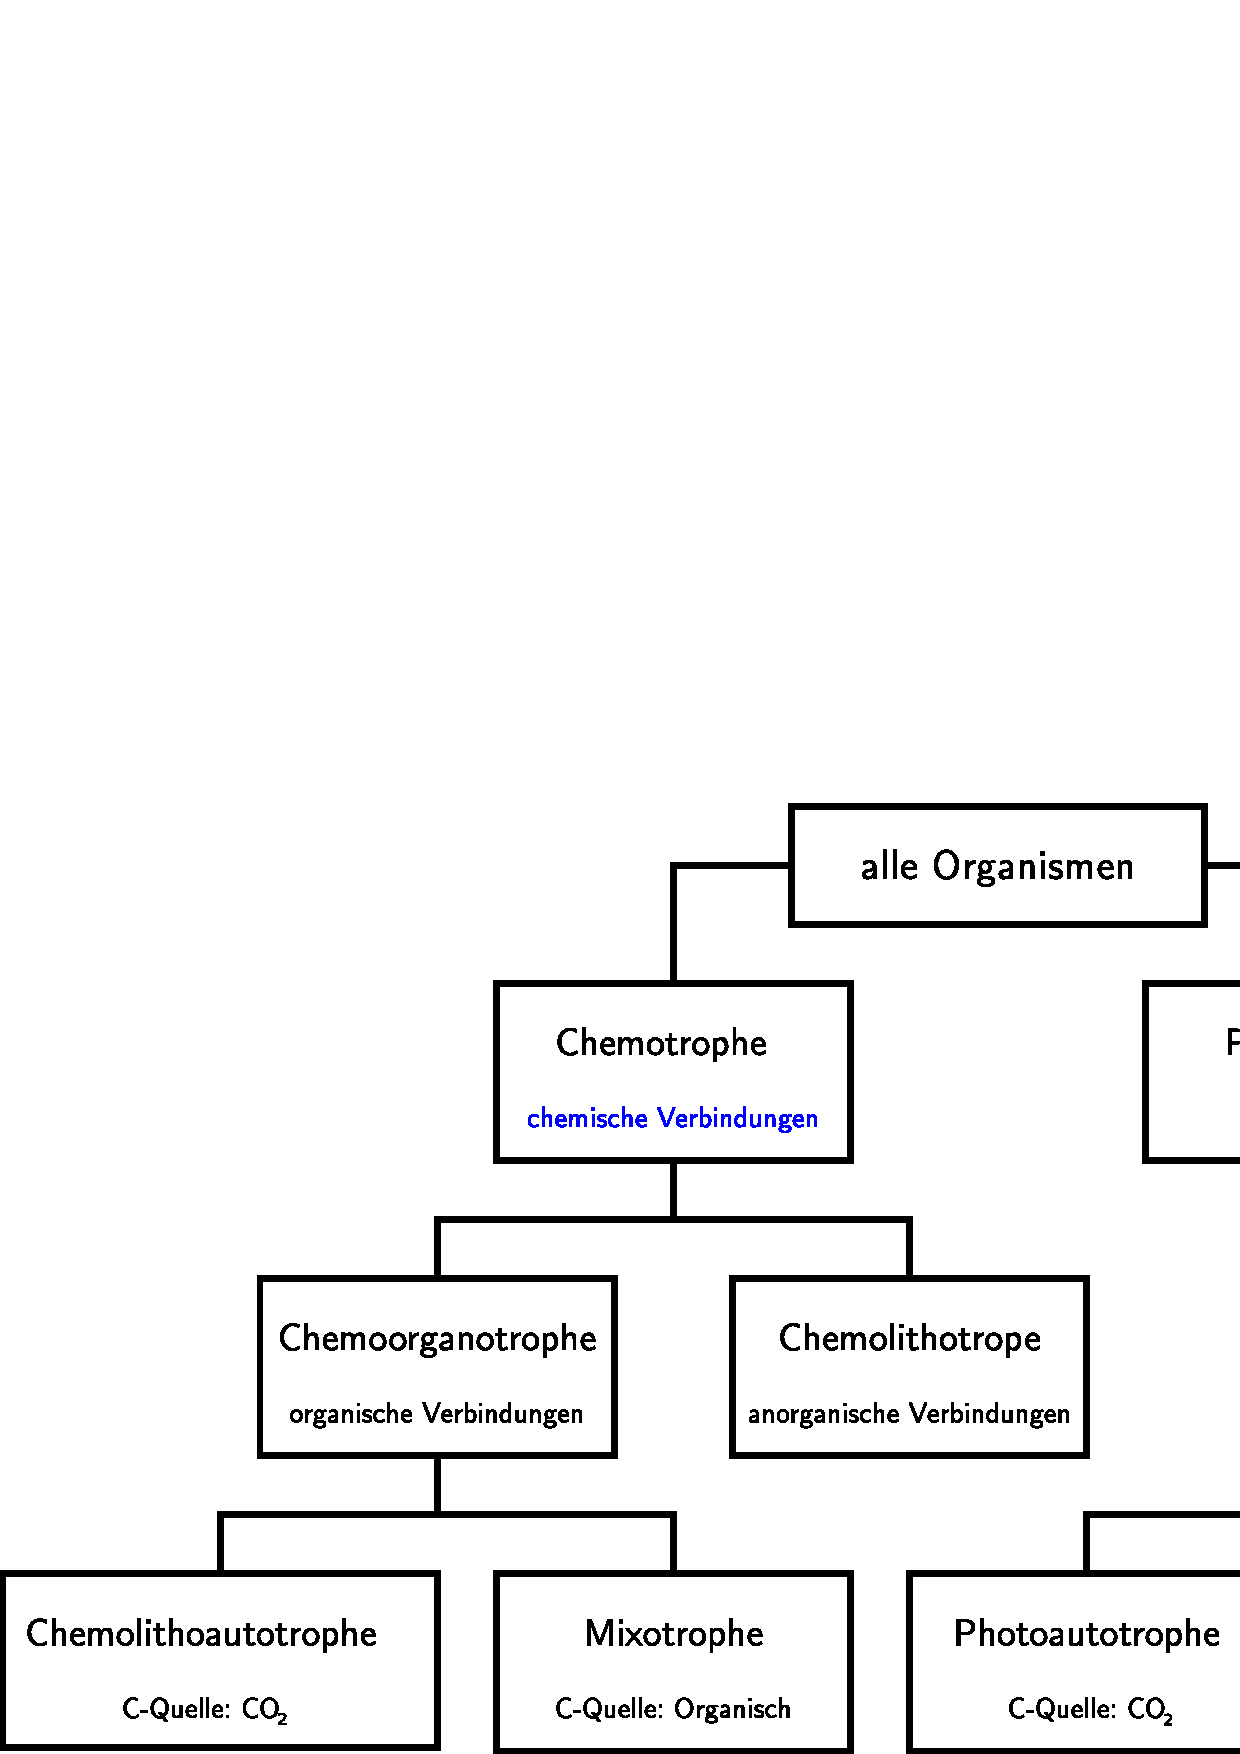
\includegraphics[scale=0.5]{./pictures/stoffwechsel.pdf}
		\end{center}
		\caption{\slshape{Stoffwechselvarianten von Mikroorganismen.
								Dargestellt sind die \textcolor{blue}{Energiequelle} und die Kohlenstoffquelle.}}
		\label{fig:Stoffwechselvarianten}
		\end{figure}

	\item[Substratkettenphosphorylierung]	\hfill	\\
		Bildung von ATP durch den direkten Transfer eines ernergiereichen
		Phosphatmoldeküls von einer phosphorylierten organischen Verbindung
		auf ADP.
\end{description}


\newpage
\bibliographystyle{apalike}
\bibliography{document}
\end{document}
\end{input}
